\documentclass{standalone}
\usepackage{tikz}
\usetikzlibrary{patterns, positioning}

\begin{document}
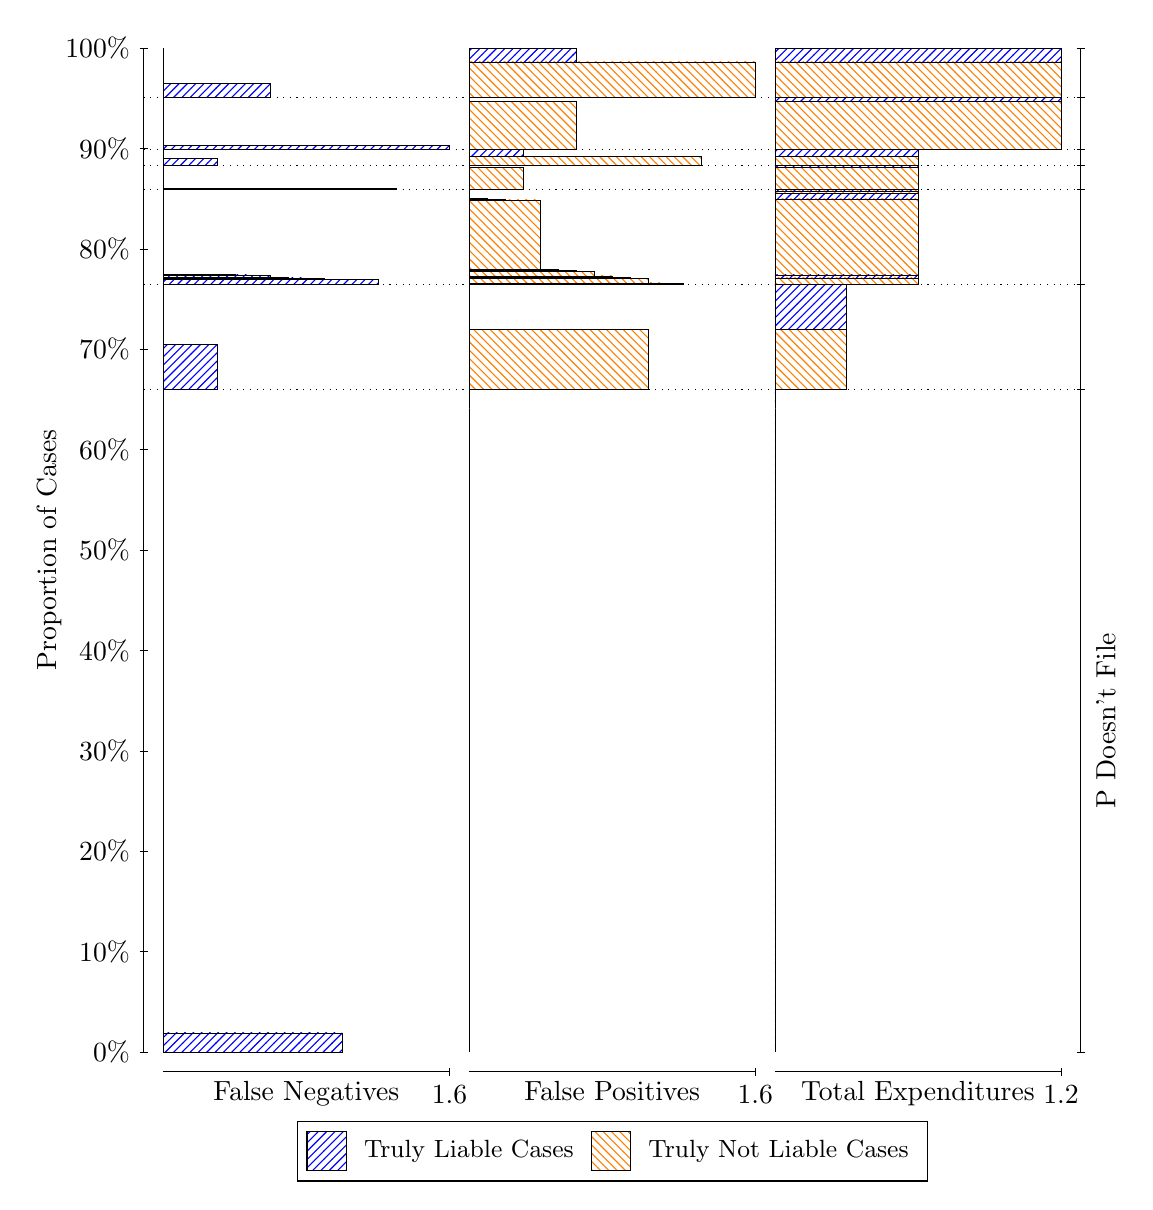
\begin{tikzpicture}
\draw[black, very thin] (1.5,1.75) -- (1.5,14.5);
\node[rotate=90, anchor=center] at (0.3, 8.125) {Proportion of Cases};
\draw[black, very thin] (1.45,1.75) -- (1.55,1.75);
\node[anchor=east] at (1.45, 1.75) {0\%};
\draw[black, very thin] (1.45,3.025) -- (1.55,3.025);
\node[anchor=east] at (1.45, 3.025) {10\%};
\draw[black, very thin] (1.45,4.3) -- (1.55,4.3);
\node[anchor=east] at (1.45, 4.3) {20\%};
\draw[black, very thin] (1.45,5.575) -- (1.55,5.575);
\node[anchor=east] at (1.45, 5.575) {30\%};
\draw[black, very thin] (1.45,6.85) -- (1.55,6.85);
\node[anchor=east] at (1.45, 6.85) {40\%};
\draw[black, very thin] (1.45,8.125) -- (1.55,8.125);
\node[anchor=east] at (1.45, 8.125) {50\%};
\draw[black, very thin] (1.45,9.4) -- (1.55,9.4);
\node[anchor=east] at (1.45, 9.4) {60\%};
\draw[black, very thin] (1.45,10.675) -- (1.55,10.675);
\node[anchor=east] at (1.45, 10.675) {70\%};
\draw[black, very thin] (1.45,11.95) -- (1.55,11.95);
\node[anchor=east] at (1.45, 11.95) {80\%};
\draw[black, very thin] (1.45,13.225) -- (1.55,13.225);
\node[anchor=east] at (1.45, 13.225) {90\%};
\draw[black, very thin] (1.45,14.5) -- (1.55,14.5);
\node[anchor=east] at (1.45, 14.5) {100\%};

\draw[black, very thin] (13.4,1.75) -- (13.4,14.5);
\draw[black, very thin] (13.35,1.75) -- (13.45,1.75);
\node[anchor=west] at (13.35, 1.75) {};
\draw[black, very thin] (13.35,10.161) -- (13.45,10.161);
\node[anchor=west] at (13.35, 10.161) {};
\draw[black, very thin] (13.35,11.501) -- (13.45,11.501);
\node[anchor=west] at (13.35, 11.501) {};
\draw[black, very thin] (13.35,12.7) -- (13.45,12.7);
\node[anchor=west] at (13.35, 12.7) {};
\draw[black, very thin] (13.35,13.008) -- (13.45,13.008);
\node[anchor=west] at (13.35, 13.008) {};
\draw[black, very thin] (13.35,13.214) -- (13.45,13.214);
\node[anchor=west] at (13.35, 13.214) {};
\draw[black, very thin] (13.35,13.87) -- (13.45,13.87);
\node[anchor=west] at (13.35, 13.87) {};
\draw[black, very thin] (13.35,14.5) -- (13.45,14.5);
\node[anchor=west] at (13.35, 14.5) {};

\draw[black, very thin, pattern color=blue, pattern=north east lines] (1.75,1.75) rectangle (4.0208,1.9915);
\draw[black, very thin, pattern color=orange, pattern=north west lines] (1.75,1.9915) rectangle (1.75,10.161);
\draw[black, very thin, pattern color=blue, pattern=north east lines] (1.75,10.161) rectangle (2.4312,10.732);
\draw[black, very thin, pattern color=orange, pattern=north west lines] (1.75,10.732) rectangle (1.75,11.501);
\draw[black, very thin, pattern color=blue, pattern=north east lines] (1.75,11.501) rectangle (4.475,11.56);
\draw[black, very thin, pattern color=blue, pattern=north east lines] (1.75,11.56) rectangle (4.2479,11.562);
\draw[black, very thin, pattern color=blue, pattern=north east lines] (1.75,11.562) rectangle (4.0208,11.565);
\draw[black, very thin, pattern color=blue, pattern=north east lines] (1.75,11.565) rectangle (3.7937,11.574);
\draw[black, very thin, pattern color=blue, pattern=north east lines] (1.75,11.574) rectangle (3.7937,11.575);
\draw[black, very thin, pattern color=blue, pattern=north east lines] (1.75,11.575) rectangle (3.5667,11.581);
\draw[black, very thin, pattern color=blue, pattern=north east lines] (1.75,11.581) rectangle (3.3396,11.586);
\draw[black, very thin, pattern color=blue, pattern=north east lines] (1.75,11.586) rectangle (3.1125,11.612);
\draw[black, very thin, pattern color=blue, pattern=north east lines] (1.75,11.612) rectangle (2.8854,11.62);
\draw[black, very thin, pattern color=blue, pattern=north east lines] (1.75,11.62) rectangle (2.6583,11.63);
\draw[black, very thin, pattern color=orange, pattern=north west lines] (1.75,11.63) rectangle (1.75,12.7);
\draw[black, very thin, pattern color=blue, pattern=north east lines] (1.75,12.7) rectangle (4.7021,12.72);
\draw[black, very thin, pattern color=orange, pattern=north west lines] (1.75,12.72) rectangle (1.75,13.008);
\draw[black, very thin, pattern color=blue, pattern=north east lines] (1.75,13.008) rectangle (2.4312,13.097);
\draw[black, very thin, pattern color=orange, pattern=north west lines] (1.75,13.097) rectangle (1.75,13.214);
\draw[black, very thin, pattern color=blue, pattern=north east lines] (1.75,13.214) rectangle (5.3833,13.264);
\draw[black, very thin, pattern color=orange, pattern=north west lines] (1.75,13.264) rectangle (1.75,13.87);
\draw[black, very thin, pattern color=blue, pattern=north east lines] (1.75,13.87) rectangle (3.1125,14.046);
\draw[black, very thin, pattern color=orange, pattern=north west lines] (1.75,14.046) rectangle (1.75,14.5);
\draw[black, very thin, pattern color=orange, pattern=north west lines] (5.6333,1.75) rectangle (5.6333,9.9197);
\draw[black, very thin, pattern color=blue, pattern=north east lines] (5.6333,9.9197) rectangle (5.6333,10.161);
\draw[black, very thin, pattern color=orange, pattern=north west lines] (5.6333,10.161) rectangle (7.9042,10.93);
\draw[black, very thin, pattern color=blue, pattern=north east lines] (5.6333,10.93) rectangle (5.6333,11.501);
\draw[black, very thin, pattern color=orange, pattern=north west lines] (5.6333,11.501) rectangle (8.3583,11.51);
\draw[black, very thin, pattern color=orange, pattern=north west lines] (5.6333,11.51) rectangle (8.1313,11.518);
\draw[black, very thin, pattern color=orange, pattern=north west lines] (5.6333,11.518) rectangle (7.9042,11.574);
\draw[black, very thin, pattern color=orange, pattern=north west lines] (5.6333,11.574) rectangle (7.6771,11.59);
\draw[black, very thin, pattern color=orange, pattern=north west lines] (5.6333,11.59) rectangle (7.45,11.606);
\draw[black, very thin, pattern color=orange, pattern=north west lines] (5.6333,11.606) rectangle (7.2229,11.668);
\draw[black, very thin, pattern color=orange, pattern=north west lines] (5.6333,11.668) rectangle (6.9958,11.68);
\draw[black, very thin, pattern color=orange, pattern=north west lines] (5.6333,11.68) rectangle (6.7687,11.684);
\draw[black, very thin, pattern color=orange, pattern=north west lines] (5.6333,11.684) rectangle (6.5417,12.572);
\draw[black, very thin, pattern color=blue, pattern=north east lines] (5.6333,12.572) rectangle (6.0875,12.581);
\draw[black, very thin, pattern color=blue, pattern=north east lines] (5.6333,12.581) rectangle (5.8604,12.589);
\draw[black, very thin, pattern color=blue, pattern=north east lines] (5.6333,12.589) rectangle (5.6333,12.7);
\draw[black, very thin, pattern color=orange, pattern=north west lines] (5.6333,12.7) rectangle (6.3146,12.989);
\draw[black, very thin, pattern color=blue, pattern=north east lines] (5.6333,12.989) rectangle (5.6333,13.008);
\draw[black, very thin, pattern color=orange, pattern=north west lines] (5.6333,13.008) rectangle (8.5854,13.125);
\draw[black, very thin, pattern color=blue, pattern=north east lines] (5.6333,13.125) rectangle (6.3146,13.214);
\draw[black, very thin, pattern color=orange, pattern=north west lines] (5.6333,13.214) rectangle (6.9958,13.82);
\draw[black, very thin, pattern color=blue, pattern=north east lines] (5.6333,13.82) rectangle (5.6333,13.87);
\draw[black, very thin, pattern color=orange, pattern=north west lines] (5.6333,13.87) rectangle (9.2667,14.324);
\draw[black, very thin, pattern color=blue, pattern=north east lines] (5.6333,14.324) rectangle (6.9958,14.5);
\draw[black, very thin, pattern color=orange, pattern=north west lines] (9.5167,1.75) rectangle (9.5167,9.9197);
\draw[black, very thin, pattern color=blue, pattern=north east lines] (9.5167,9.9197) rectangle (9.5167,10.161);
\draw[black, very thin, pattern color=orange, pattern=north west lines] (9.5167,10.161) rectangle (10.425,10.93);
\draw[black, very thin, pattern color=blue, pattern=north east lines] (9.5167,10.93) rectangle (10.425,11.501);
\draw[black, very thin, pattern color=orange, pattern=north west lines] (9.5167,11.501) rectangle (11.333,11.58);
\draw[black, very thin, pattern color=blue, pattern=north east lines] (9.5167,11.58) rectangle (11.333,11.619);
\draw[black, very thin, pattern color=orange, pattern=north west lines] (9.5167,11.619) rectangle (11.333,12.584);
\draw[black, very thin, pattern color=blue, pattern=north east lines] (9.5167,12.584) rectangle (11.333,12.657);
\draw[black, very thin, pattern color=orange, pattern=north west lines] (9.5167,12.657) rectangle (11.333,12.685);
\draw[black, very thin, pattern color=blue, pattern=north east lines] (9.5167,12.685) rectangle (11.333,12.7);
\draw[black, very thin, pattern color=orange, pattern=north west lines] (9.5167,12.7) rectangle (11.333,12.989);
\draw[black, very thin, pattern color=blue, pattern=north east lines] (9.5167,12.989) rectangle (11.333,13.008);
\draw[black, very thin, pattern color=orange, pattern=north west lines] (9.5167,13.008) rectangle (11.333,13.125);
\draw[black, very thin, pattern color=blue, pattern=north east lines] (9.5167,13.125) rectangle (11.333,13.214);
\draw[black, very thin, pattern color=orange, pattern=north west lines] (9.5167,13.214) rectangle (13.15,13.82);
\draw[black, very thin, pattern color=blue, pattern=north east lines] (9.5167,13.82) rectangle (13.15,13.87);
\draw[black, very thin, pattern color=orange, pattern=north west lines] (9.5167,13.87) rectangle (13.15,14.324);
\draw[black, very thin, pattern color=blue, pattern=north east lines] (9.5167,14.324) rectangle (13.15,14.5);
\draw[black, dotted] (1.5,10.161) -- (13.4,10.161);
\draw[black, dotted] (1.5,11.501) -- (13.4,11.501);
\draw[black, dotted] (1.5,12.7) -- (13.4,12.7);
\draw[black, dotted] (1.5,13.008) -- (13.4,13.008);
\draw[black, dotted] (1.5,13.214) -- (13.4,13.214);
\draw[black, dotted] (1.5,13.87) -- (13.4,13.87);
\draw[black, very thin] (1.75,1.5) -- (5.3833,1.5);
\node[anchor=north] at (3.5667, 1.5) {False Negatives};
\draw[black, very thin] (5.3833,1.45) -- (5.3833,1.55);
\node[anchor=north] at (5.3833, 1.45) {1.6};

\draw[black, very thin] (5.6333,1.5) -- (9.2667,1.5);
\node[anchor=north] at (7.45, 1.5) {False Positives};
\draw[black, very thin] (9.2667,1.45) -- (9.2667,1.55);
\node[anchor=north] at (9.2667, 1.45) {1.6};

\draw[black, very thin] (9.5167,1.5) -- (13.15,1.5);
\node[anchor=north] at (11.333, 1.5) {Total Expenditures};
\draw[black, very thin] (13.15,1.45) -- (13.15,1.55);
\node[anchor=north] at (13.15, 1.45) {1.2};

\node[black, centered, rotate=90] at (13.72, 5.9556) {P Doesn't File};







\draw (7.449999999999999,1.5) node[draw=none] (baseCoordinate) {};
\begin{scope}[align=center]
        \matrix[scale=0.5, draw=black, below=0.5cm of baseCoordinate, nodes={draw}, column sep=0.1cm]{
            \node[rectangle, draw, minimum width=0.5cm, minimum height=0.5cm, pattern=north east lines, pattern color=blue] {}; &
            \node[draw=none, font=\small] (B) {Truly Liable Cases}; &
            \node[rectangle, draw, minimum width=0.5cm, minimum height=0.5cm, pattern=north west lines, pattern color=orange] {}; &
            \node[draw=none, font=\small] (B) {Truly Not Liable Cases}; \\
            };
\end{scope}

\end{tikzpicture}
\end{document}